\documentclass[a4paper,norsk, 10pt]{article}
\usepackage[utf8]{inputenc}
\usepackage{verbatim}
\usepackage{listings}
\usepackage{graphicx}
\usepackage[norsk]{babel}
\usepackage{a4wide}
\usepackage{color}
\usepackage{amsmath}
\usepackage{float}
\usepackage{amssymb}
\usepackage[dvips]{epsfig}
\usepackage[toc,page]{appendix}
\usepackage[T1]{fontenc}
\usepackage{cite} % [2,3,4] --> [2--4]
\usepackage{shadow}
\usepackage{hyperref}
\usepackage{titling}
\usepackage{marvosym }
%\usepackage{subcaption}
\usepackage{subfig}
\usepackage[noabbrev]{cleveref}
\usepackage{cite}
\usepackage{todonotes}

\setlength{\droptitle}{-10em}   % This is your set screw

\setcounter{tocdepth}{2}

\lstset{language=c++}
\lstset{alsolanguage=[90]Fortran}
\lstset{alsolanguage=Python}
\lstset{basicstyle=\small}
\lstset{backgroundcolor=\color{white}}
\lstset{frame=single}
\lstset{stringstyle=\ttfamily}
\lstset{keywordstyle=\color{red}\bfseries}
\lstset{commentstyle=\itshape\color{blue}}
\lstset{showspaces=false}
\lstset{showstringspaces=false}
\lstset{showtabs=false}
\lstset{breaklines}
\title{AST5220 Milestone 3}
\author{Daniel Heinesen, daniehei}
\begin{document}
\maketitle

\section{Introduction}
Now having found  how the Universe expands and how the coupling of electrons and photons influences the free mean path -- optical path -- of the photons. This means that we are ready to look at how initial perturbations in the Universe evolve. We will do this by integrating the Einstein-Boltzmann equations (see sec. \ref{sec:theory}) from an initial time deep in the radiation dominated era, well before decoupling, until today. Having integrated these equation for the scalar metric perturbations $\Phi$ and $\Psi$, the density perturbations of dark matter and baryons $\delta$ and $\delta_b$ and the velocity of dark matter and baryons $v$ and $v_b$, we can look at the different Fourier modes and learn how different scales are affected.

\section{Theory}\label{sec:theory}

\subsection{Normal Integration}\label{sec:normal}
One can show that the Einstein-Boltzmann equation for the quantities we are interested in is given as

\begin{equation}
\Theta_0 ' = -\frac{ck}{\mathcal{H}}\Theta_1 - \Phi',
\end{equation}
\begin{equation}
\Theta_1' = \frac{ck}{3\mathcal{H}}\Theta_0 - \frac{2ck}{3\mathcal{H}}\Theta_2 + \frac{ck}{3\mathcal{H}}\Psi + \tau'\left[\Theta_1 + \frac{1}{3}v_b\right],
\end{equation}
\begin{equation}
\Theta_l' = \frac{lck}{(2l+1)\mathcal{H}}\Theta_{l-1} - \frac{(l+1)ck}{(2l+1)\mathcal{H}}\Theta_{l+1} + \tau'\left[\Theta_l - \frac{1}{10}\Theta_l \delta_{l,2}\right],\qquad 2 \leq l < l_{max}
\end{equation}
\begin{equation}
\Theta_l' = \frac{ck}{\mathcal{H}}\Theta_{l-1} - c\frac{l+1}{\mathcal{H}\eta(x)}\Theta_l + \tau'\Theta_l, \qquad l = l_{max}
\end{equation}
\begin{equation}
\delta' = \frac{ck}{\mathcal{H}}v - 3\Phi',
\end{equation}
\begin{equation}
v' = -v - \frac{ck}{\mathcal{H}}\Psi,
\end{equation}
\begin{equation}
\delta_b' = \frac{ck}{\mathcal{H}}v_b -3\Phi',
\end{equation}
\begin{equation}
v_b' = -v_b - \frac{ck}{\mathcal{H}}\Psi + \tau' R(3\Theta_1 + v_b),
\end{equation}
\begin{equation}
\Phi' = \Psi - \frac{c^2k^2}{3\mathcal{H}^2}\Phi + \frac{H_0^2}{2\mathcal{H}^2}\left[\Omega_ma^{-1}\delta + \Omega_b a^{-1}\delta_b + 4\Omega_r\Theta_0 a^{-2}\right],
\end{equation}
\begin{equation}
\Psi = -\Phi - \frac{12H_0^2}{c^2k^2a^2}\Omega_r\Theta_2,
\end{equation}
\begin{equation}
R = \frac{4\Omega_r}{3\Omega_b a}.
\end{equation}
All of the above equations are in Fourier space, with wave number $k$. This means that we can look at how the perturbations at different Fourier modes evolve (independently), which corresponds to different scales with $\lambda \propto k^{-1}$. We now have the differential equations we need to integrate, but to be able to do that we need initial conditions. We will start our integration a long time ago, when the particle horizon was extremely small compared to all modes $k$, which means $k\eta << 1$. With this it is possible to get initial conditions as functions of $\Phi$
\begin{equation}
\Phi = 1,
\end{equation}
\begin{equation}
\delta = \delta_b = \frac{3}{2}\Phi,
\end{equation}
\begin{equation}
v = v_b = \frac{ck}{2\mathcal{H}}\Phi,
\end{equation}
\begin{equation}
\Theta_0 = \frac{1}{2}\Phi,
\end{equation}
\begin{equation}
\Theta_1 = -\frac{ck}{6\mathcal{H}}\Phi,
\end{equation}
\begin{equation}
\Theta_2 = -\frac{20ck}{45\mathcal{H}\tau'}\Theta_1,
\end{equation}
\begin{equation}
\Theta_l = -\frac{l}{2l+1}\frac{ck}{\mathcal{H}\tau'}\Theta_{l-1}.
\end{equation}
Just setting $\Phi = 1$ may seem odd, but we are through inflation only able to get the initial power spectrum of $\Phi$. But thankfully we do not need to worry about that before after we have integrated. We can, in other word, just set the initial value of $\Phi$ as we wish, integrate everything and then multiply by the power spectrum of $\Phi$ after the integration. This gives the same result as if we would have gotten if we just the power spectrum as the initial value. 

An other ting to notice is that we have defined a $l_{max}$, while $l$ in reality can take an infinite number of values. This is because we can use a technique called \textit{line of sight integration}, where only the first six $l$s are needed to find the rest \todo{Is this the correct way of defining line of sight integration?}.


\subsection{Tight Coupling}\label{sec:tight}
There is one period we need to be careful of. At early times, before recombination, the mean free path of the photons are really small, meaning that $\tau >> 1$. During this time photons are unable to travel far before being scattered by electrons, this makes the photon aware only of a small area around it. This means that the baryons and photons are tightly coupled, behaving more like a single fluid. Due to the coupling, all but the largest perturbation are smoothed out, leaving the fluid in near equilibrium. All momentums of the photon temperatures are therefore negligible, except from $\Theta_0$ and $\Theta_1$. This is all well and fine, except from the fact that we now have a $\tau'$ which is very large multiplied with a factor $3\Theta_1-v_b$ which is very small. This is a recipe for numerical instability. This means that we need another way of integrating during this period. One can show that with these limitations we can integrate most of the expressions as before, but need to change $v_b'$ and $\Theta_0'$ to

\begin{equation}
v_b' = \frac{1}{1+R}\left[-v_b - \frac{ck}{\mathcal{H}}\Psi + R(q + \frac{ck}{\mathcal{H}}(-\Theta_0 + 2\Theta_2) - \frac{ck}{\mathcal{H}}\Psi)\right],
\end{equation}
\begin{equation}
\Theta_0' = \frac{1}{3}(q - v_b'),
\end{equation}
where 
\begin{equation}
q = \frac{-[(1-2R)\tau' + (1+R)\tau''](3\Theta_1 + v_b) - \frac{ck}{\mathcal{H}}\Psi + (1-\frac{\mathcal{H}'}{\mathcal{H}})\frac{ck}{\mathcal{H}}(-\Theta_0 + 2\Theta_2) - \frac{ck}{\mathcal{H}}\Theta_0'}{(1+R)\tau' + \frac{\mathcal{H}'}{\mathcal{H}} - 1}.
\end{equation}
With these we can calculate the other momenta as
\begin{equation}
\Theta_2 = \frac{-20ck}{45\mathcal{H}\tau'}\Theta_1,
\end{equation}
\begin{equation}
\Theta_l = -\frac{l}{2l+1}\frac{ck}{\mathcal{H}\tau'}\Theta_{l-1}
\end{equation}

So when will we use the tight coupling functions. We are going to define tight coupling as ending when either $|\tau'| < 10$ or $\left|\frac{ck}{\mathcal{H}\tau'}\right|>0.1$ or recombination have happened.

\section{Method}
Having the differential equations and initial values we can now begin to integrate. We want to integrate the equations from $x = \ln a_{init} = \ln 10^{-8}$ until today, where $x_0 = 0$. Since we know that different eras are more sensitive to numerical instability, we will make a x-grid with different step sizes. Before recombination we will have $1000$ grid points, during recombination we will use $200$ grid points, and $300$ grid points between the end of recombination and now. 

Since all the Fourier modes are independent, we can integrate them one by one. For this report only six such modes are used: $k = 0.1, 8.4, 85.9, 245.1, 636.8, 1000 c/H_0$. This is to demonstrate the physics at different scales.  

For each $k$ we start by finding at which value of $x$ tight coupling ends. We then use the the equations found in sec. \ref{sec:tight} during the integration. Note that only $\Theta_0$ and $\Theta_1$ are integrated here, the rest of the momenta are just algebraic expressions. When tight coupling is over, we can instead start to use the differential equations from sec. \ref{sec:normal}. 

All the integration is done by an integration function from \textit{Numerical Recipes} with a Bulirsch-Stoer stepper.

Since the $x$ value of the end of tight coupling is different for each $k$, this value has to be calculated for each $k$. Arrays with all the relevant quantities are saved after each step, for later visualization.

\todo{The method seems short, but I do not know what else to write.}

\section{Results}

\begin{figure*}[!htbp]
\centering
\begin{tabular}{@{}ccc@{}}
\subfloat[Survival function for the different treatments. We see that there is some difference, with patients treated with the placebo having lower survival during most of the study. But the difference is very small.\label{fig:delta}]{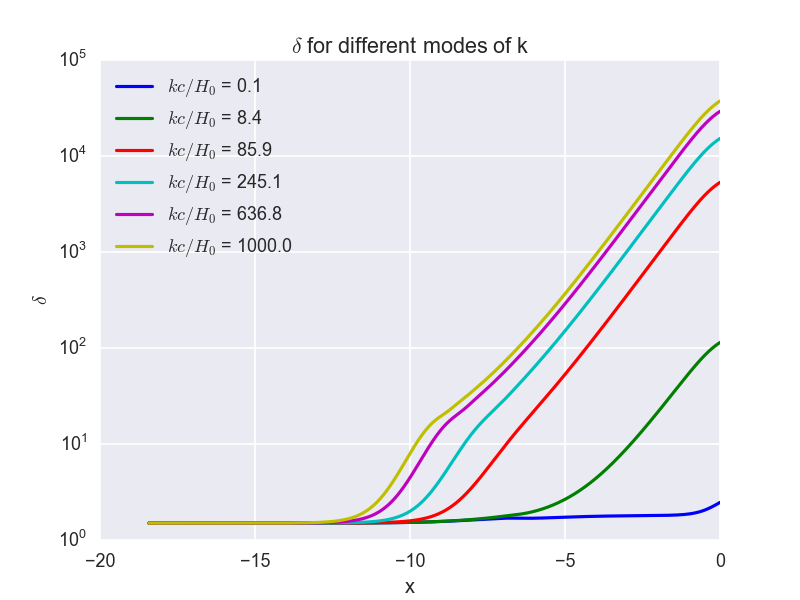
\includegraphics[width=0.5\textwidth]{delta.png}} & 
\subfloat[The figure shows that the survival for male patients are smaller than that for the female patients. The difference is not large, and may not be significant.\label{fig:delta_b}]{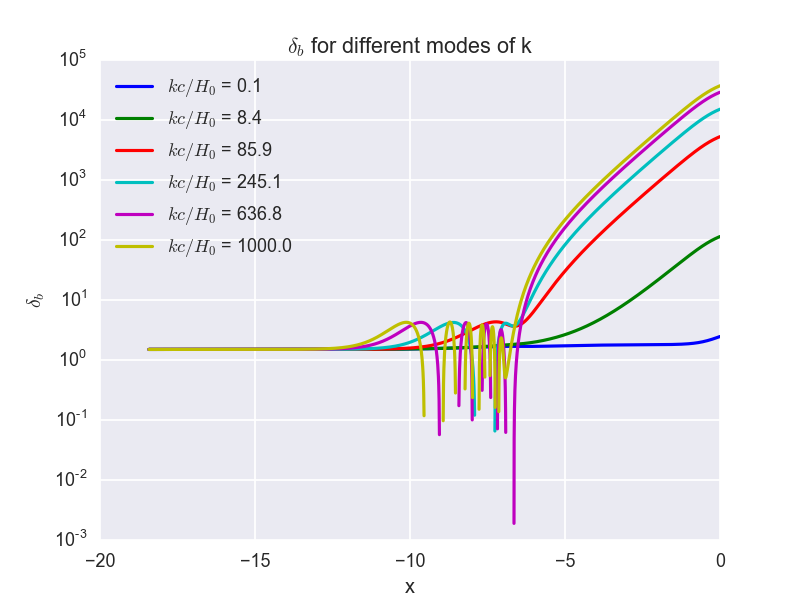
\includegraphics[width=0.5\textwidth]{delta_b.png}} \\
\subfloat[The figure shows that there is a large difference in the survival based on the severity of the ascites of the patient at the start of the observation. The more fluid the patient has, the lower the survival.\label{fig:v}]{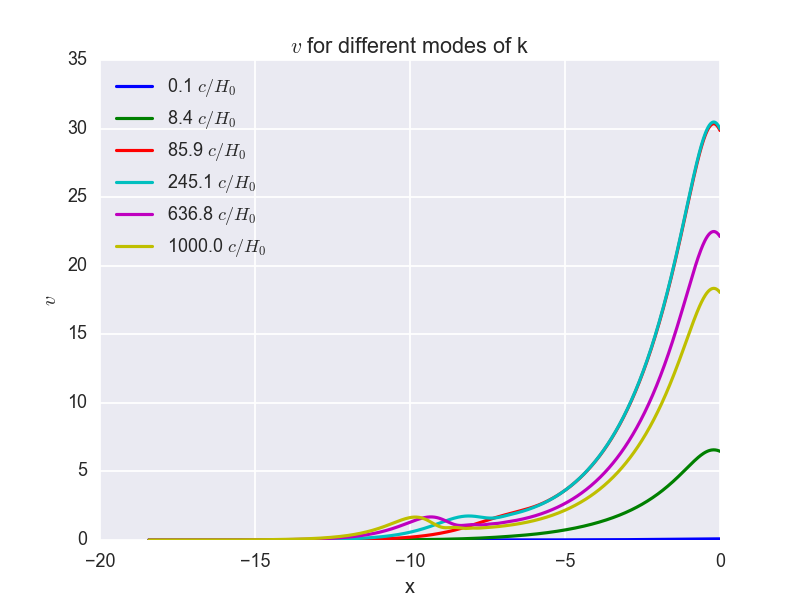
\includegraphics[width=0.5\textwidth]{v.png}} &
\subfloat[The figure shows that the age plays a important role in the survival, with older patients surviving shorter than the younger ones.\label{fig:v_b}]{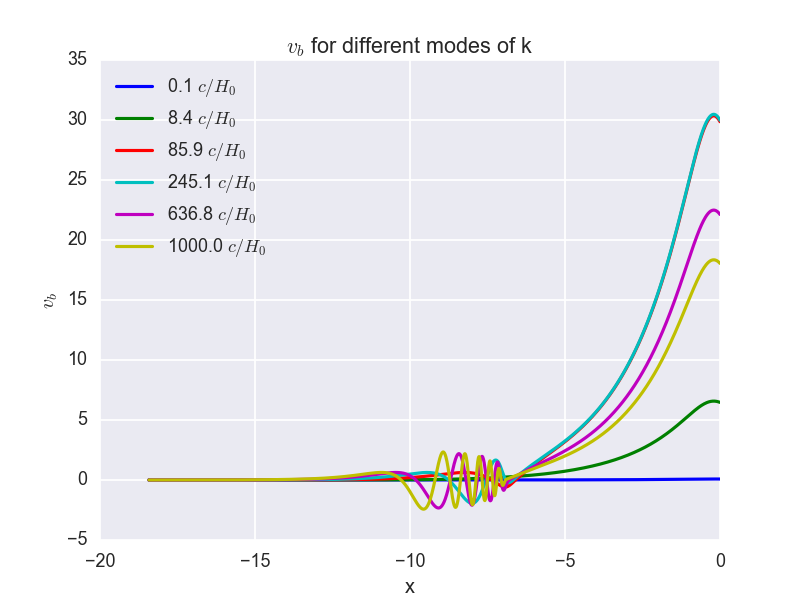
\includegraphics[width=0.5\textwidth]{v_b.png}} 
\end{tabular}
\caption[]{Four figure showing the estimated survival function for different groups.}
\label{fig:delta_v}
\end{figure*}


\begin{figure*}[!htbp]
\centering
\begin{tabular}{@{}ccc@{}}
\subfloat[Survival function for the different treatments. We see that there is some difference, with patients treated with the placebo having lower survival during most of the study. But the difference is very small.\label{fig:Psi}]{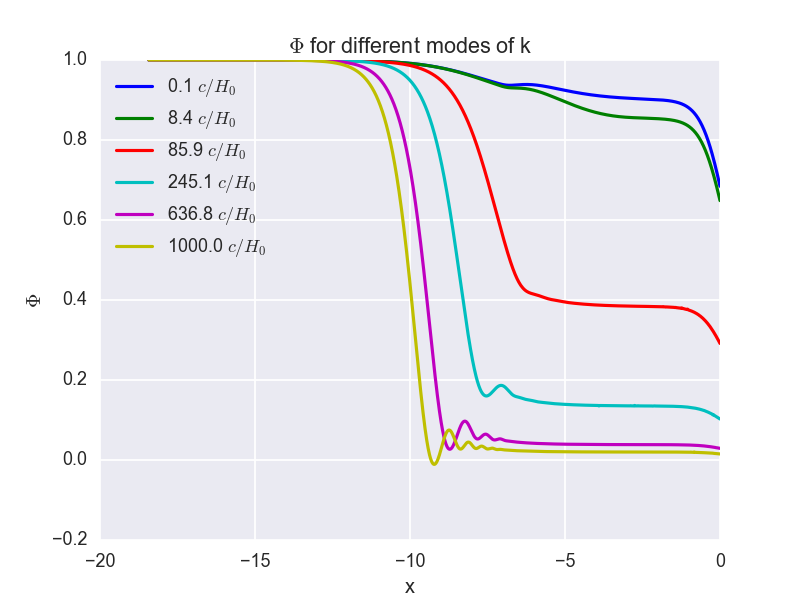
\includegraphics[width=0.5\textwidth]{Phi.png}} & 
\subfloat[The figure shows that the survival for male patients are smaller than that for the female patients. The difference is not large, and may not be significant.\label{fig:Psi}]{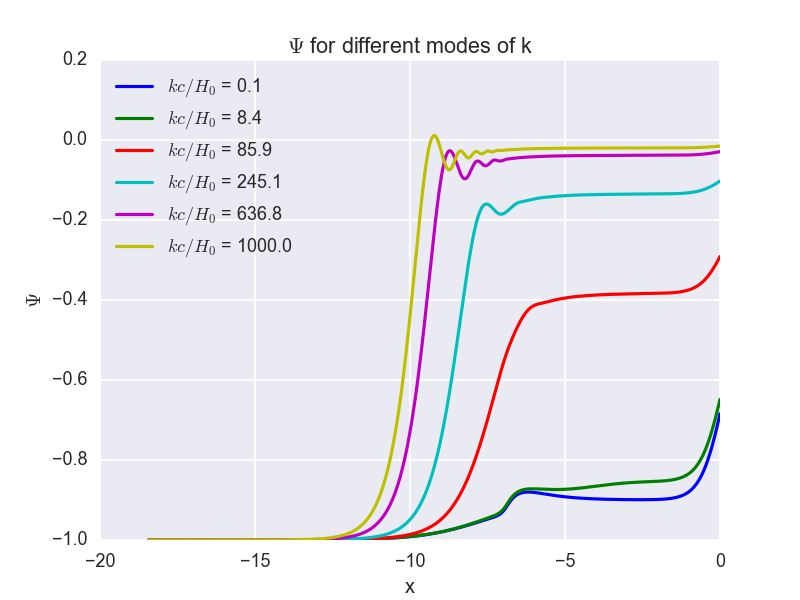
\includegraphics[width=0.5\textwidth]{Psi.png}} 
\end{tabular}
\caption[]{Four figure showing the estimated survival function for different groups.}
\label{fig:psi_phi}
\end{figure*}


\begin{figure}
\centering
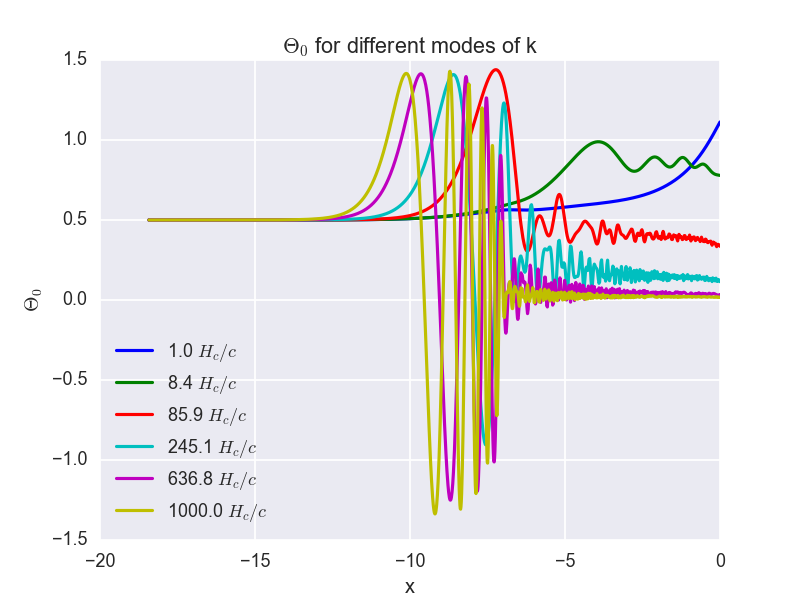
\includegraphics[scale=0.5]{Theta_0.png}
\caption{•}\label{fig:theta}
\end{figure}

\todo[inline]{Notes: As Psi crosses $a_eq$ the transfer function decreases the Psi that have not crossed the horizon to 9/10. If Psi crosses the horizon in the matter dominated regime, it stays constant. This is no longer the case when dark energy takes over, thus the dip in the end (described by the growth function). Growth function is independent of $k$, and is very small in dark energy dom., and we therefore see that perturbations flattens out near $x=0$.

In matter era. delta goes as a. In rad. dom. they grows as well but not as prominent(meszaros suppression). The pressure from the radiation slows the perturbations down, but as matter begins to dominate, the pressure weakens and the perturbations grow faster.

In rad. dom. the potential is determined by photons, and not dark matter. DM is instead determined by the potential. Potential decays in rad dom.

Seems that modes grows independent of $k$ after crossing the horizon.

The oscillations found in $\Theta_0$ is that makes $\delta_b$ oscillate, due to tight coupling.

Due to pressure of 



The oscillations in baryon plots are acoustic oscillations. This is because with only baryons, the perturbations goes as a cosine (from extra galactic)}

\end{document}

